\documentclass[xcolor=dvipsnames]{beamer}

\usepackage{ub-beamer}
\usepackage[overlay,absolute]{textpos}
\usepackage{multimedia}
\usepackage{graphicx}
\usepackage{soul}
\usepackage[dvipsnames]{xcolor}
\usepackage{colortbl}
\DeclareGraphicsExtensions{.png,.jpg,.pdf}
\usepackage{float}
\usepackage{amsmath}
\usepackage{tikz}
\usetikzlibrary{arrows,positioning}
\definecolor{links}{HTML}{2A1B81}
\hypersetup{colorlinks,linkcolor=,urlcolor=links}
\usepackage[printwatermark]{xwatermark}
\usepackage{color}
\usepackage[absolute,overlay]{textpos}
\usepackage{listings}
\usepackage{amssymb}
\usepackage{pifont}

\newcommand\YAMLcolonstyle{\color{red}\mdseries}
\newcommand\YAMLkeystyle{\color{black}\bfseries}
\newcommand\YAMLvaluestyle{\color{blue}\mdseries}

\lstset{
  keywords={true,false,null,y,n},
  keywordstyle=\color{darkgray}\bfseries,
  basicstyle=\ttfamily\bfseries\tiny\YAMLkeystyle, % assuming a key comes first
  sensitive=false,
  comment=[l]{\#},
  morecomment=[s]{/*}{*/},
  commentstyle=\color{purple}\ttfamily,
  stringstyle=\YAMLvaluestyle\ttfamily,
  moredelim=[l][\color{orange}]{\&},
  moredelim=[l][\color{magenta}]{*},
  moredelim=**[il][\YAMLcolonstyle{:}\YAMLvaluestyle]{:}, % switch to value style at :
  morestring=[b]',
  morestring=[b]",
  literate =    {---}{{\ProcessThreeDashes}}3
                {>}{{\textcolor{red}\textgreater}}1     
                {|}{{\textcolor{red}\textbar}}1 
                {\ -\ }{{\mdseries\ -\ }}3,
}

\newcommand\ProcessThreeDashes{\llap{\color{cyan}\mdseries-{-}-}}
\newcommand{\cmark}{\ding{51}}%
\newcommand{\xmark}{\ding{55}}%
\newcommand{\presentationDate}{24th October 2017}



\title[Automating and publishing workflow analyses in Galaxy]{Towards automating and publishing workflow analyses in Galaxy}



\author[Andrea Bagnacani]{
  \texorpdfstring{Andrea Bagnacani}{Andrea Bagnacani}
}



\institute[University of Rostock]{
  Dept.$\,$ of Systems Biology \& Bioinformatics\newline
  University of Rostock, Rostock (Germany)
}



\date[Bielefeld \presentationDate]{
  Bielefeld, \presentationDate
}

\subject{workflow, reusability, publishing, Galaxy}



\begin{document}

%
% presentation page
%
\begin{frame}[noframenumbering,plain]
  \titlepage
\end{frame}


%
% summary page
%
\newcommand{\one}{From data to information}
\newcommand{\two}{The Galaxy framework}
\newcommand{\three}{A platform for training}
\newcommand{\four}{de.STAIR}
\newcommand{\five}{Conclusions}
\begin{frame}
  \frametitle{Summary}
  \begin{itemize}
    \item \one
    \item \two
    \item \three
    \item \four
    \item \five
  \end{itemize}
\end{frame}



%
% information in data-driven science
%
\begin{frame}
  \frametitle{\one}
  Life Sciences have become more and more data-driven.\newline\newline
  Insights on biological problems are gained leveraging on computational approaches:
  \vspace{0.2cm}
  \begin{itemize}
    \item collecting data through experiments or simulations
    \item structuring data into data-sets
    \item analyzing data leveraging on multidisciplinary approaches
    \item sharing protocols and best practices to reproduce results
  \end{itemize}
  \vspace{0.2cm}
  These approaches enable researchers to put data into context, and obtain workflows for further investigation and reproducibility.
\end{frame}

\begin{frame}
  \frametitle{\one}
  Life Sciences have become more and more data-driven.\newline\newline
  Insights on biological problems are gained leveraging on computational approaches:
  \vspace{0.2cm}
  \begin{itemize}
    \item collecting data through experiments or simulations \textcolor{ForestGreen}{\cmark}
    \item structuring data into data-sets \textcolor{ForestGreen}{\cmark}
    \item analyzing data leveraging on multidisciplinary approaches \textcolor{ForestGreen}{\cmark}
    \item sharing protocols and best practices to reproduce results \textcolor{BrickRed}{\xmark}
  \end{itemize}
  \vspace{0.2cm}
  However, the novelty of such approaches requires an effort for the promotion of standards, and ease of availability and reproducibility.
  % such efforts usually find their home within active and vibrant communities
\end{frame}



%
% the galaxy framework
%
\begin{frame}
  \frametitle{\two}
  \framesubtitle{a web-based framework}
  \vspace{-0.2cm}
  \begin{center}
    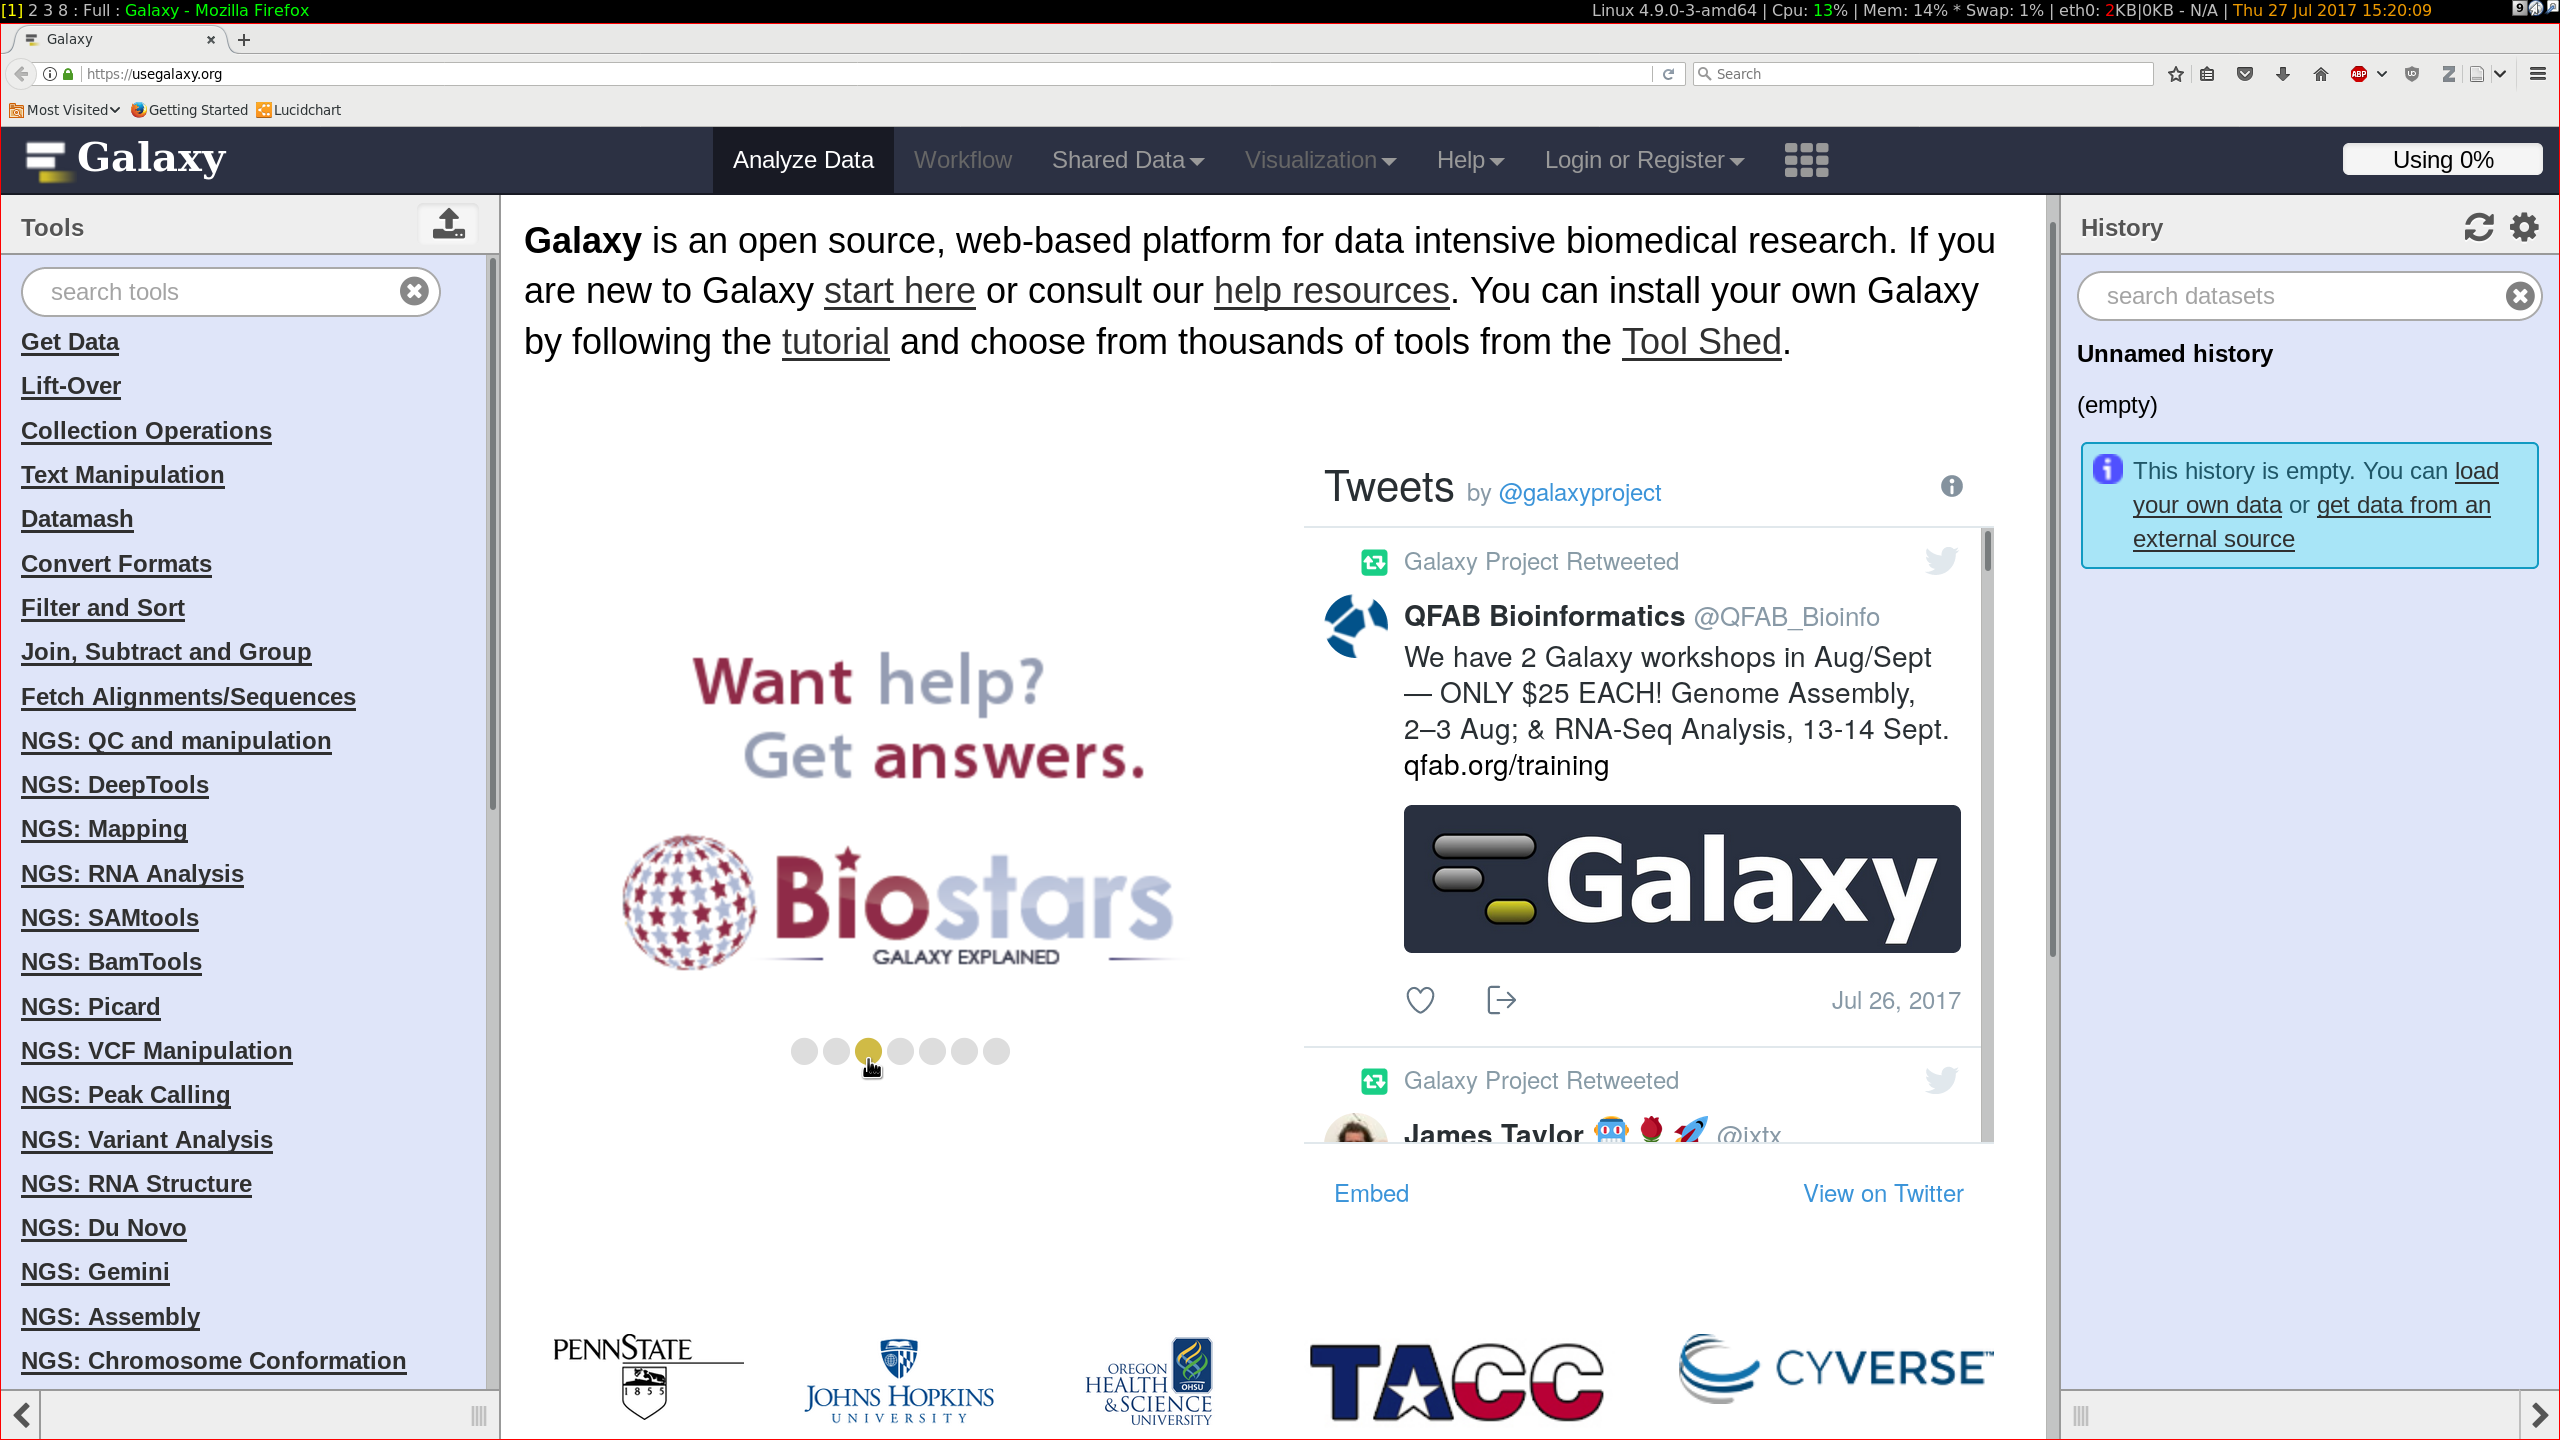
\includegraphics[width=0.80\textwidth]{images/screenshot_usegalaxy}
  \end{center}
  Galaxy is a web framework for computational bio/medical research
  \begin{itemize}
    \item public/private online/offline instances
    \item domain specific
  \end{itemize}
\end{frame}

\begin{frame}
  \frametitle{\two}
  \framesubtitle{Operations}
  \vspace{-0.2cm}
  \begin{center}
    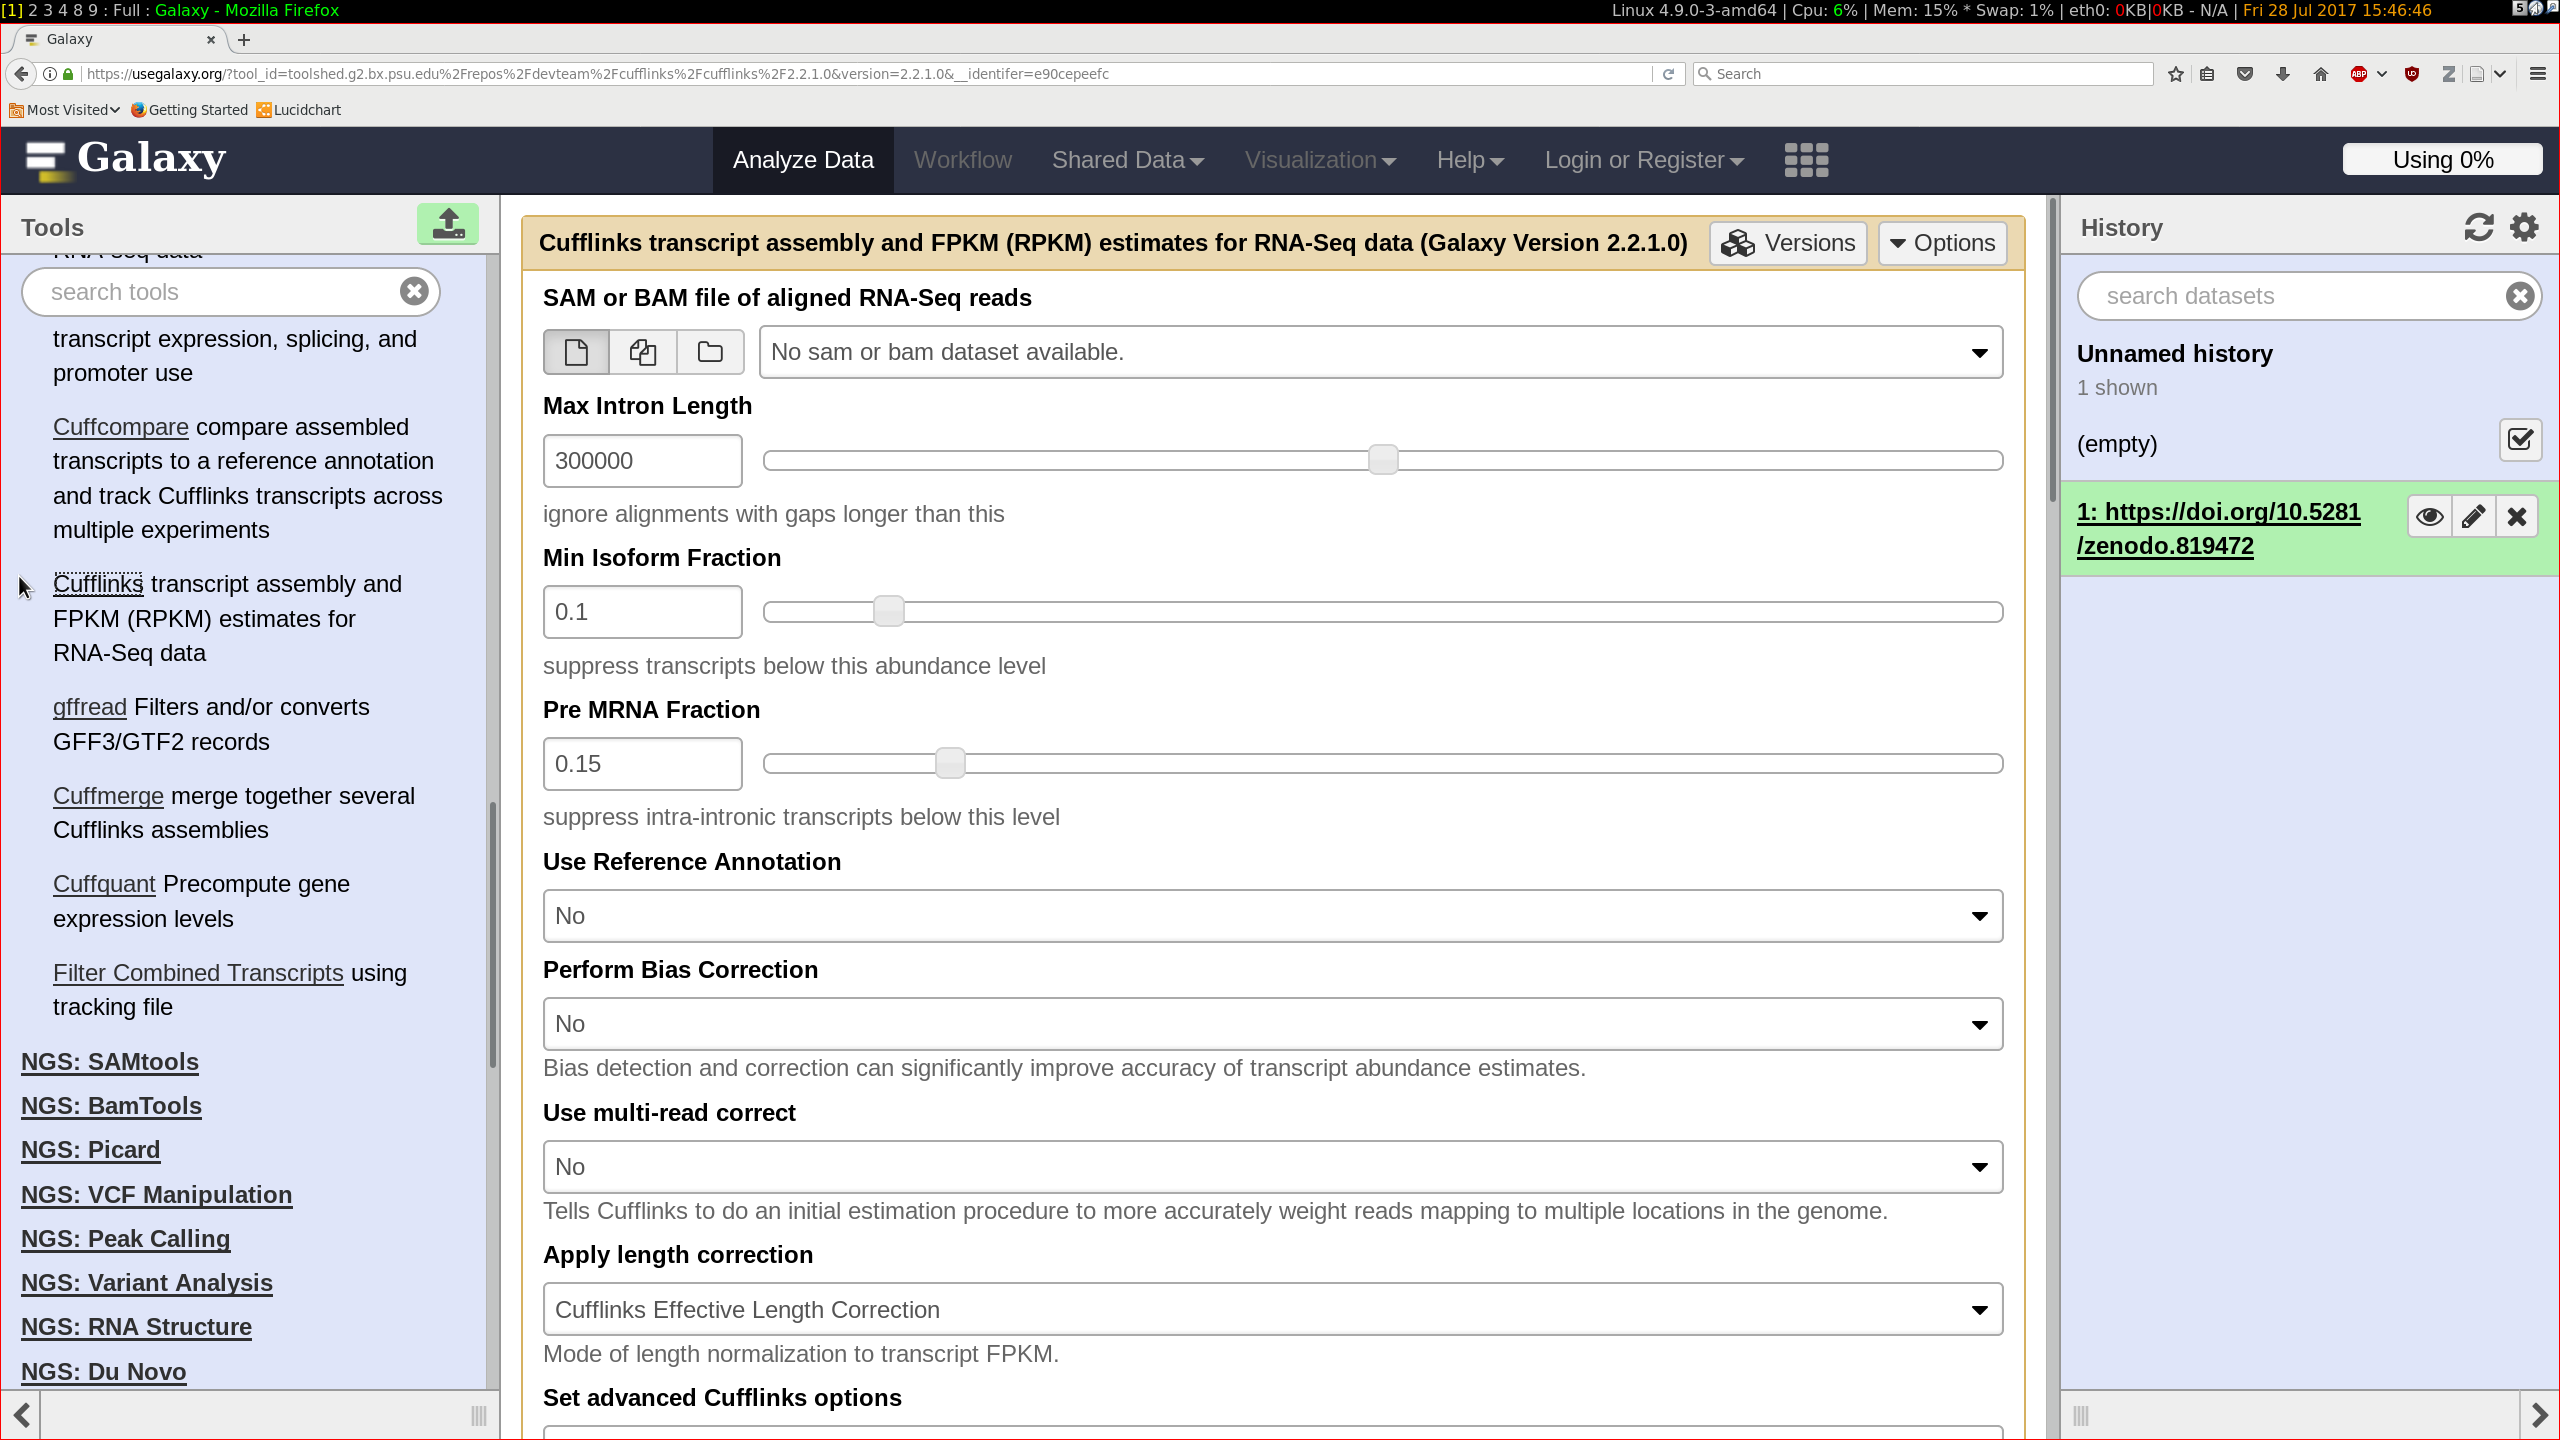
\includegraphics[width=0.80\textwidth]{images/screenshot_usegalaxy_cufflinks}
  \end{center}
  Galaxy is a web framework for computational bio/medical research
  \begin{itemize}
    \item tools can be searched, parametrized, and applied on a dataset
    \item a history of data and operations is kept for tracking/reuse
  \end{itemize}
\end{frame}

\begin{frame}
  \frametitle{\two}
  \framesubtitle{Sharable workflows}
  \vspace{-0.2cm}
  \begin{center}
    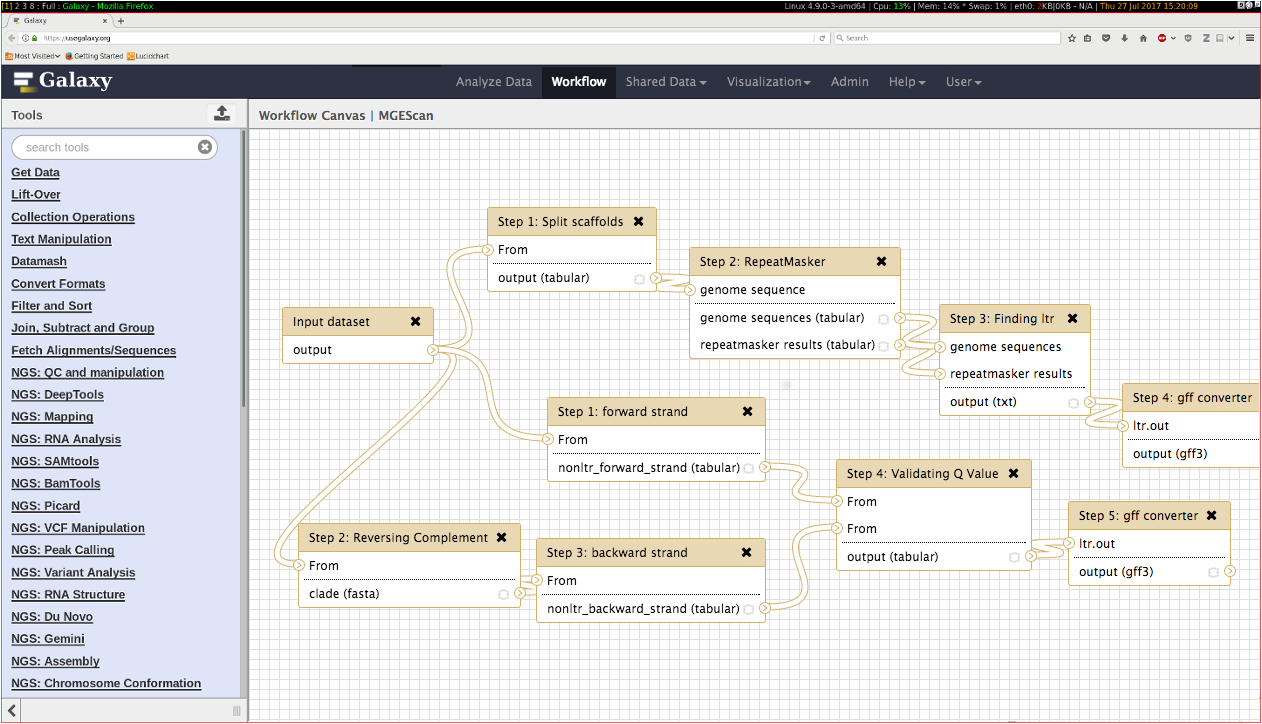
\includegraphics[width=0.80\textwidth]{images/screenshot_usegalaxy_workflow}
  \end{center}
  Galaxy is a web framework for computational bio/medical research
  \begin{itemize}
    \item histories can be exported to graphical workflows
    \item workflows can be shared, edited, and run for replication
  \end{itemize}
\end{frame}

\begin{frame}
  \frametitle{\two}
  \framesubtitle{Interactive tours}
  \vspace{-0.2cm}
  \begin{center}
    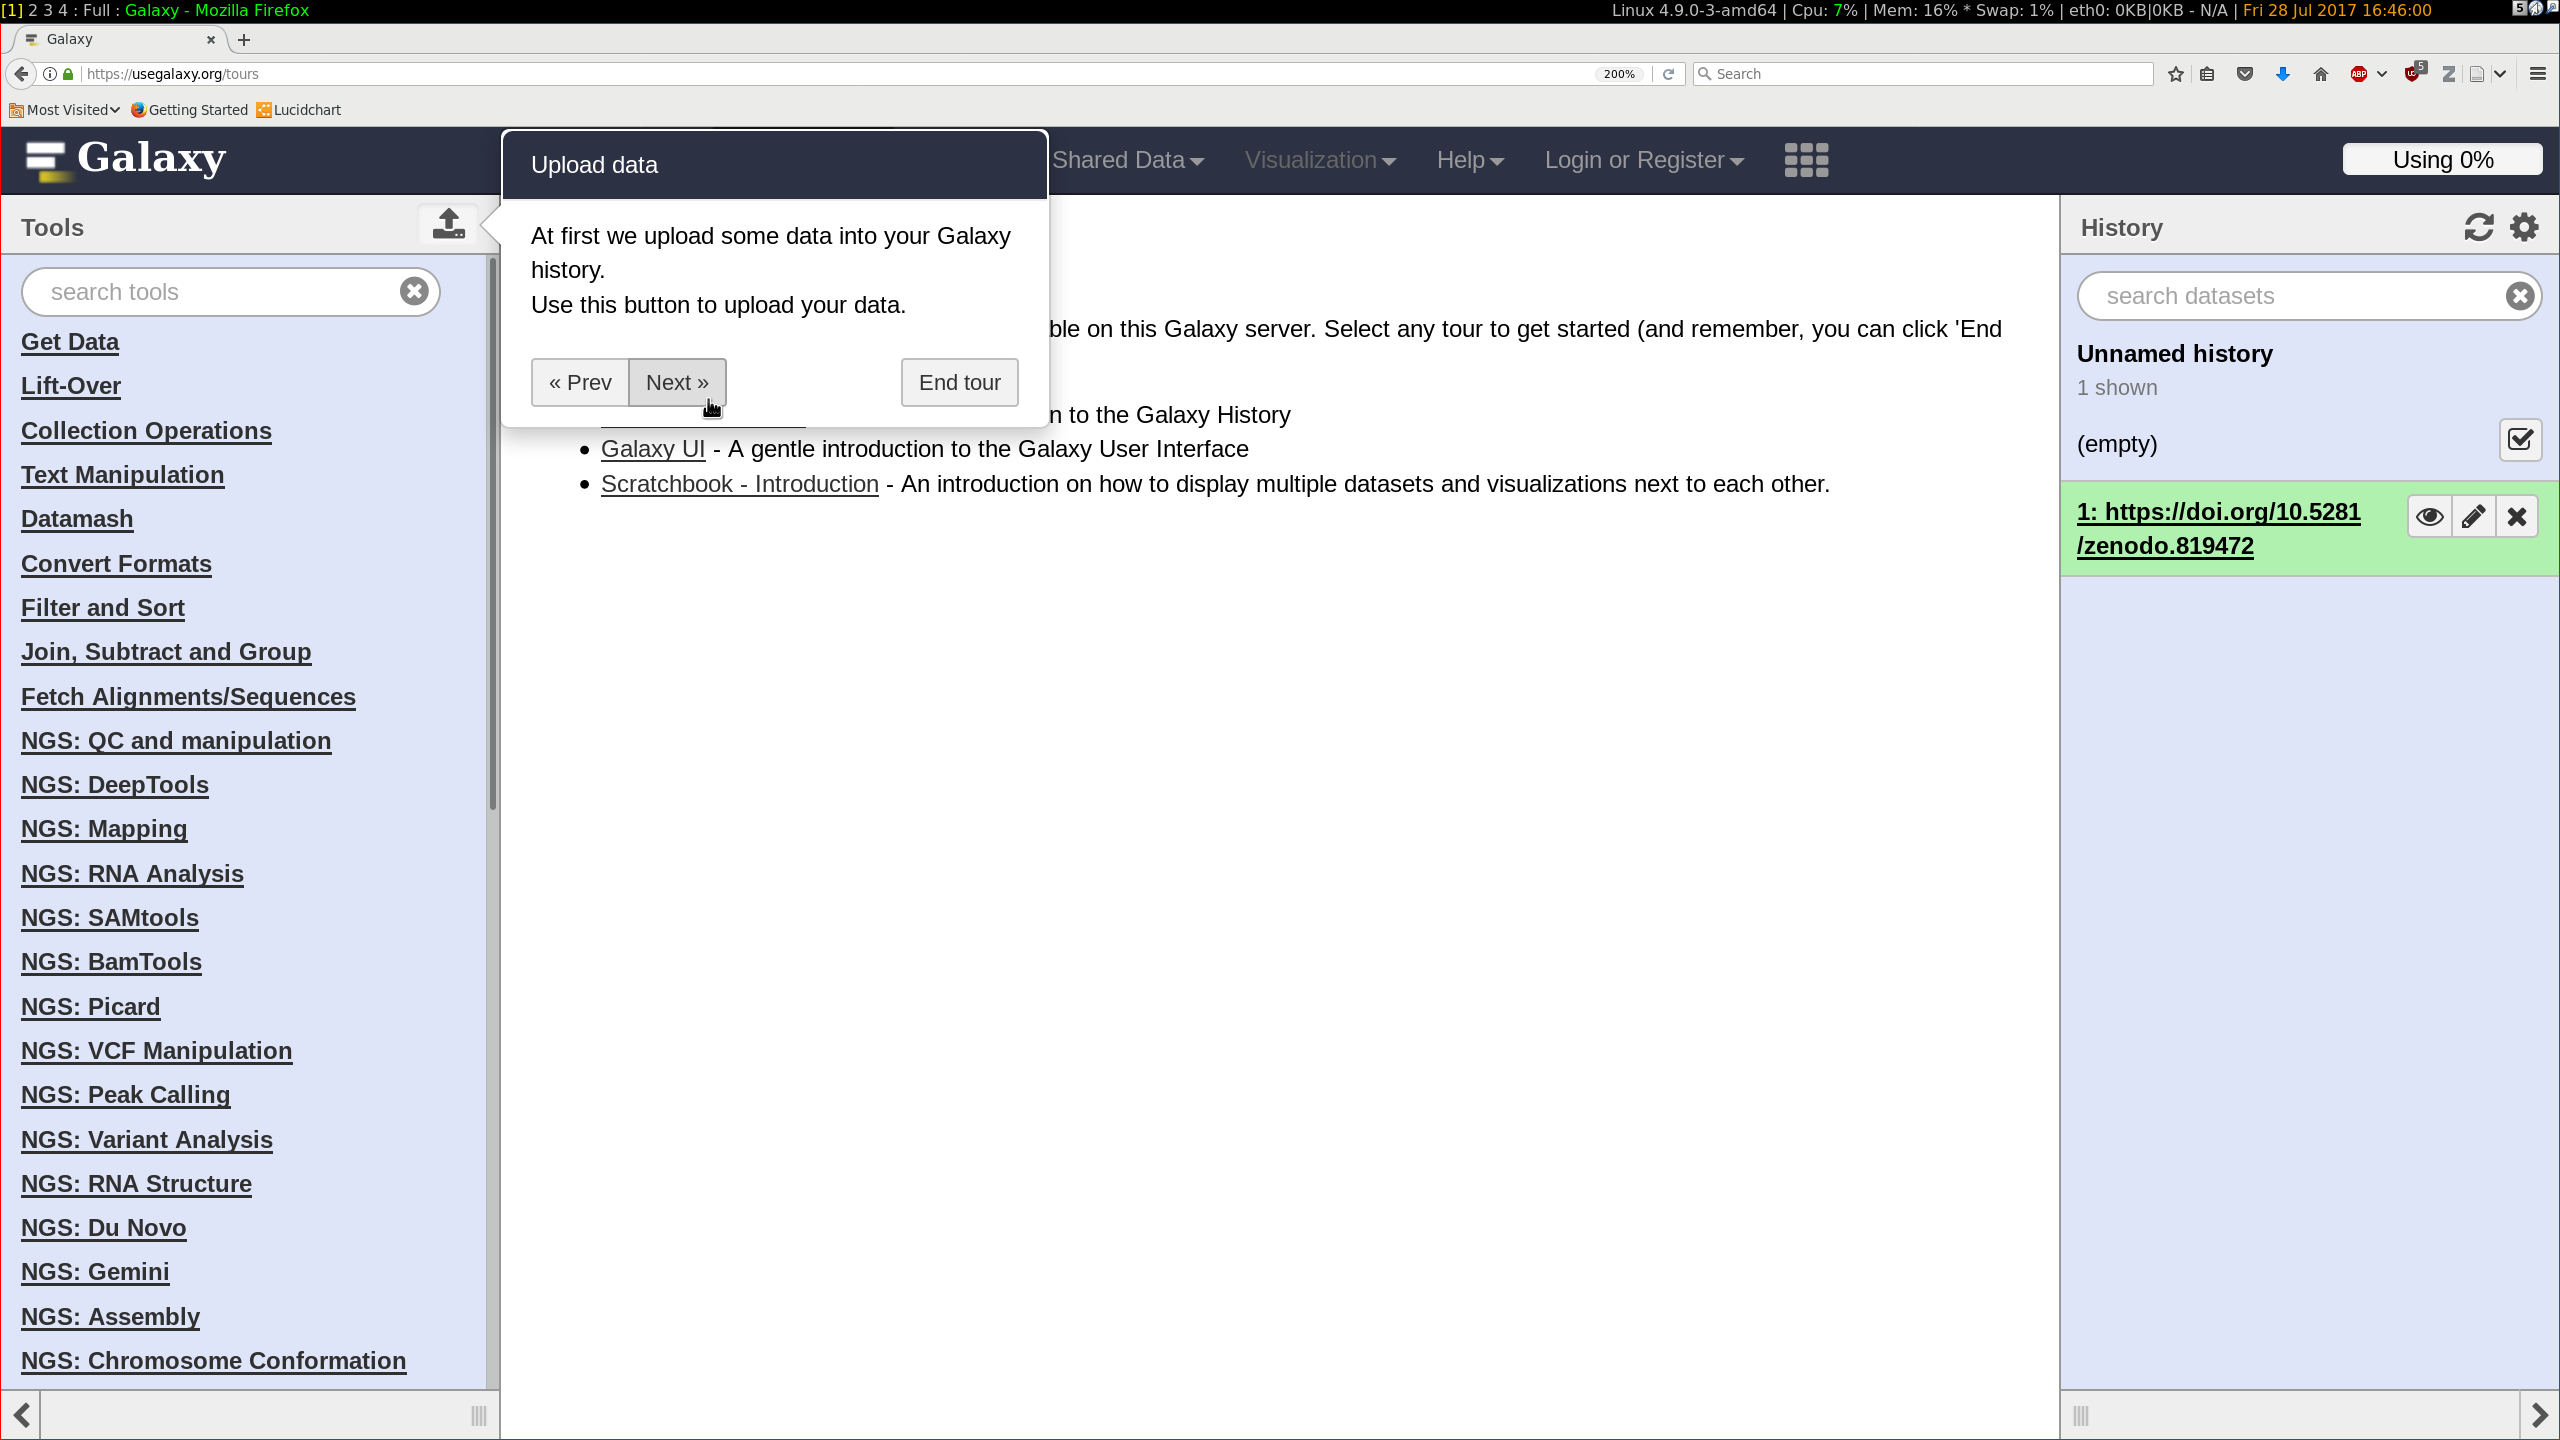
\includegraphics[width=0.80\textwidth]{images/screenshot_usegalaxy_tours}
  \end{center}
  Galaxy is a web framework for computational bio/medical research
  \begin{itemize}
    \item interactive tours can guide users through its interface
    \item tours can be created for any topic, for showcase or guidance
  \end{itemize}
\end{frame}

\begin{frame}[fragile]
  \frametitle{\two}
  \framesubtitle{Interactive tours - behind the scenes}
  Tours are YAML files, containing dialogues' text, position, and click actions
  \begin{lstlisting}
    id: galaxy_ui
    name: Galaxy UI
    description: A gentle introduction to the Galaxy User Interface
    title_default: Welcome to Galaxy

    # A tour is made of several steps, each of them beginning with a dash '-'
    steps:
      # 'title's will be displayed in the header of each step-container
      # If you don't specify any title, a default title is used, defined above.
      - title: Welcome to Galaxy
        # 'content' is the actual text that is shown to the user
        content: This short tour guides you through the Galaxy user interface.<br/>
        backdrop: true

      # 'element' is the JQuery Selector of the element you want to describe
      - title: Upload your data
        element: ".upload-button"
        intro: Galaxy supports many ways to get in your data.<br>
               Use this button to upload your data.
        # position of the text box relative to the selected element
        position: right
        # You can trigger click() events on arbitrary elements before (preclick)
        # or after (postclick) the element is shown
        postclick:
          - .upload-button

  \end{lstlisting}
\end{frame}



%
% a platform for training
%
\begin{frame}
  \frametitle{\three}
  \begin{center}
    
\includegraphics[width=0.30\textwidth]{images/logo_gtn}
  \end{center}
  The \href{https://galaxyproject.github.io/training-material/}{Galaxy Training Network} is a collection of tutorials for researchers, developers, and admins leveraging on the Galaxy framework for deliver or provide answers to bio/medical research.\newline
  \begin{columns}
    \begin{column}{0.5\textwidth}
      \scriptsize{
        \begin{itemize}
          \item Galaxy interface
          \item Proteomics
          \item Assembly
          \item ChIP-Seq data analysis
          \item Variant analysis
          \item Sequence analysis
        \end{itemize}
      }
    \end{column}
    \begin{column}{0.5\textwidth}
      \scriptsize{
        \begin{itemize}
          \item Transcriptomics
          \item Epigenetics
          \item Metagenomics
          \item Server administration
          \item Training the trainers
          \item Galaxy development
        \end{itemize}
      }
    \end{column}
  \end{columns}
\end{frame}

\begin{frame}
  \frametitle{\three}
  \begin{center}
    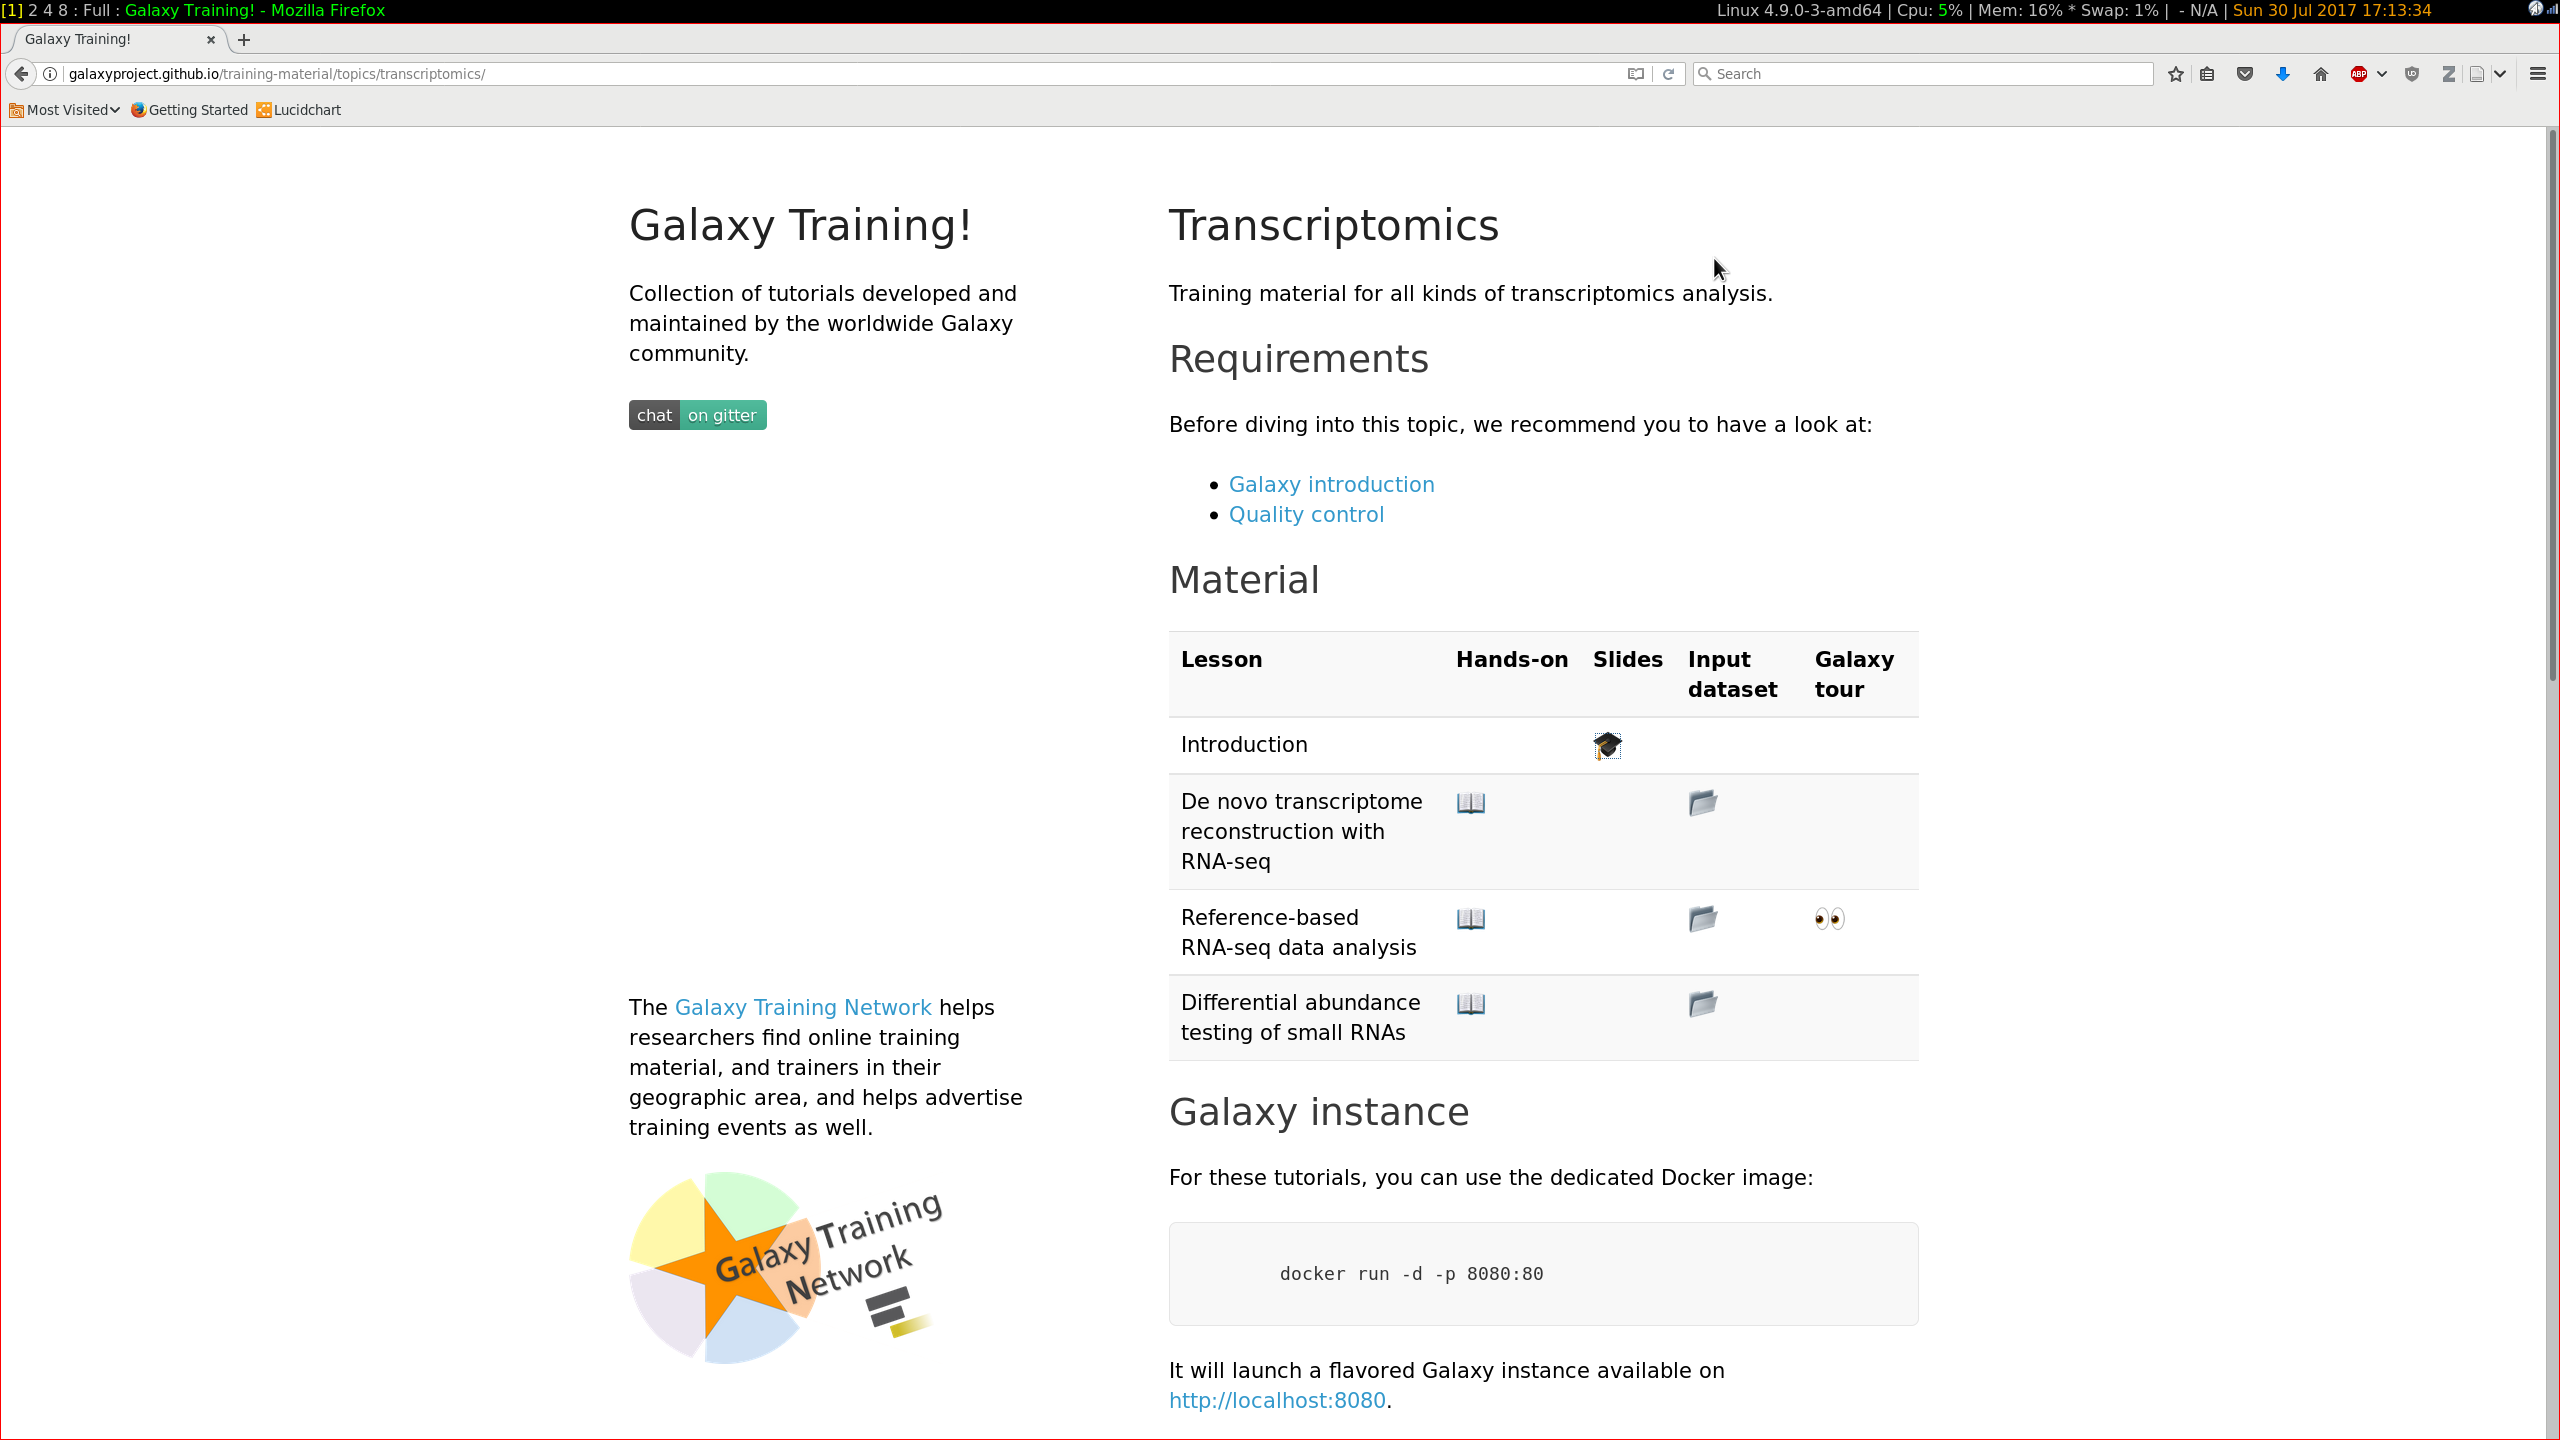
\includegraphics[width=0.90\textwidth]{images/screenshot_usegalaxy_training}
  \end{center}
  \vspace{-0.3cm}
  Each training topic contains multiple examples, available as:
  \begin{itemize}
    \item hands-on material with example datasets
    \item slides
    \item interactive tours
  \end{itemize}
\end{frame}



%
% de.STAIR
%
{
  \usebackgroundtemplate{
    \tikz\node[opacity=0.09]{
    \parbox[c][\paperheight][c]{\paperwidth}{\centering
\includegraphics[scale=0.7]{images/logo_destair}}
    };
  }
\begin{frame}
  \frametitle{\four}
  \framesubtitle{From where we start}
  Life Sciences have become more and more data-driven.\newline\newline
  Insights on biological problems are gained leveraging on computational approaches:
  \vspace{0.2cm}
  \begin{itemize}
    \item collecting data through experiments or simulations \textcolor{ForestGreen}{\cmark}
    \item structuring data into data-sets \textcolor{ForestGreen}{\cmark}
    \item analyzing data leveraging on multidisciplinary approaches \textcolor{ForestGreen}{\cmark}
    \item sharing protocols and best practices to reproduce results \textcolor{ForestGreen}{\cmark}
  \end{itemize}
  \vspace{0.2cm}
  Galaxy is able to cover all these requirements for carrying out reproducuble best-practices in data-driven research.\newline\newline
  However, new problems require new workflows, and the workflow collection might be too restrictive to address them.
\end{frame}
}

\begin{frame}
  \frametitle{\four}
  \framesubtitle{Recommendation system}
  \begin{itemize}
    \item Reusing the idea of the interactive tours, we can provide the user alternative tools to carry out their analyses.
  \end{itemize}
  \begin{itemize}
    \item This approach allows for modular workflows, enabling the inclusion of alternative/experimental tools to carry out similar operations within new workflows.
  \end{itemize}
  \vspace{0.5cm}
  To do so, Galaxy needs a \emph{recommendation system} able to suggest tools to its users, and load them on-demand to build and allow flexible workflows.
\end{frame}

\begin{frame}
  \frametitle{\four}
  \framesubtitle{Recommendation system}
  Behind the interface, the idea is that of enabling users to decide which \emph{path} to walk towards the completion of their own analysis.
  \vspace{-0.2cm}
  \begin{center}
    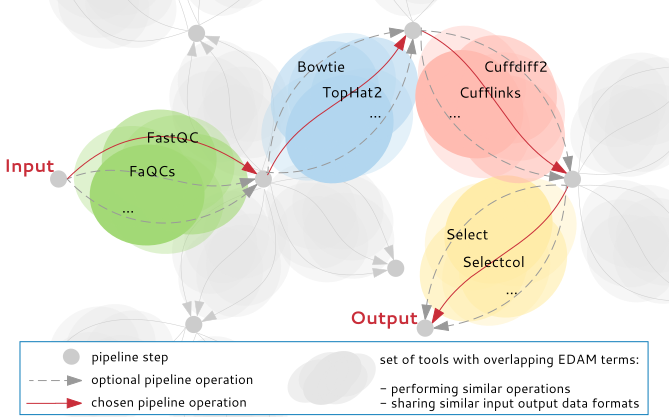
\includegraphics[width=0.80\textwidth]{images/recommendation_system}
  \end{center}
\end{frame}

\begin{frame}
  \frametitle{\four}
  \framesubtitle{Recommendation system}
  Behind the interface, the idea is that of enabling users to decide which \emph{path} to walk towards the completion of their own analysis.\newline\newline
  What is needed:
  \vspace{0.1cm}
  \begin{itemize}
    \item group tools on the basis of their grade of overlap in carrying out a specific functionality
    \item define a set of input and output file formats at the immediate begin and end of each tool's operation
    \item define tags (trajectories throughout the possible steps) like RNA-Seq analysis, Epigenetic analysis, ...
    \item equip Galaxy with an interactive-tour-like dialog system that embeds the aforementionned recommendations to propose solutions within the available set of tools
  \end{itemize}
\end{frame}

\begin{frame}
  \frametitle{\four}
  \framesubtitle{Recommendation system}
  To group tools in categories of operations and in/out file formats, we will rely on \href{https://bio.tools}{bio.tools}, a registry of tools whose operation and formats are described by means of the \href{https://github.com/edamontology/edamontology}{EDAM Ontology}.
  \begin{center}
    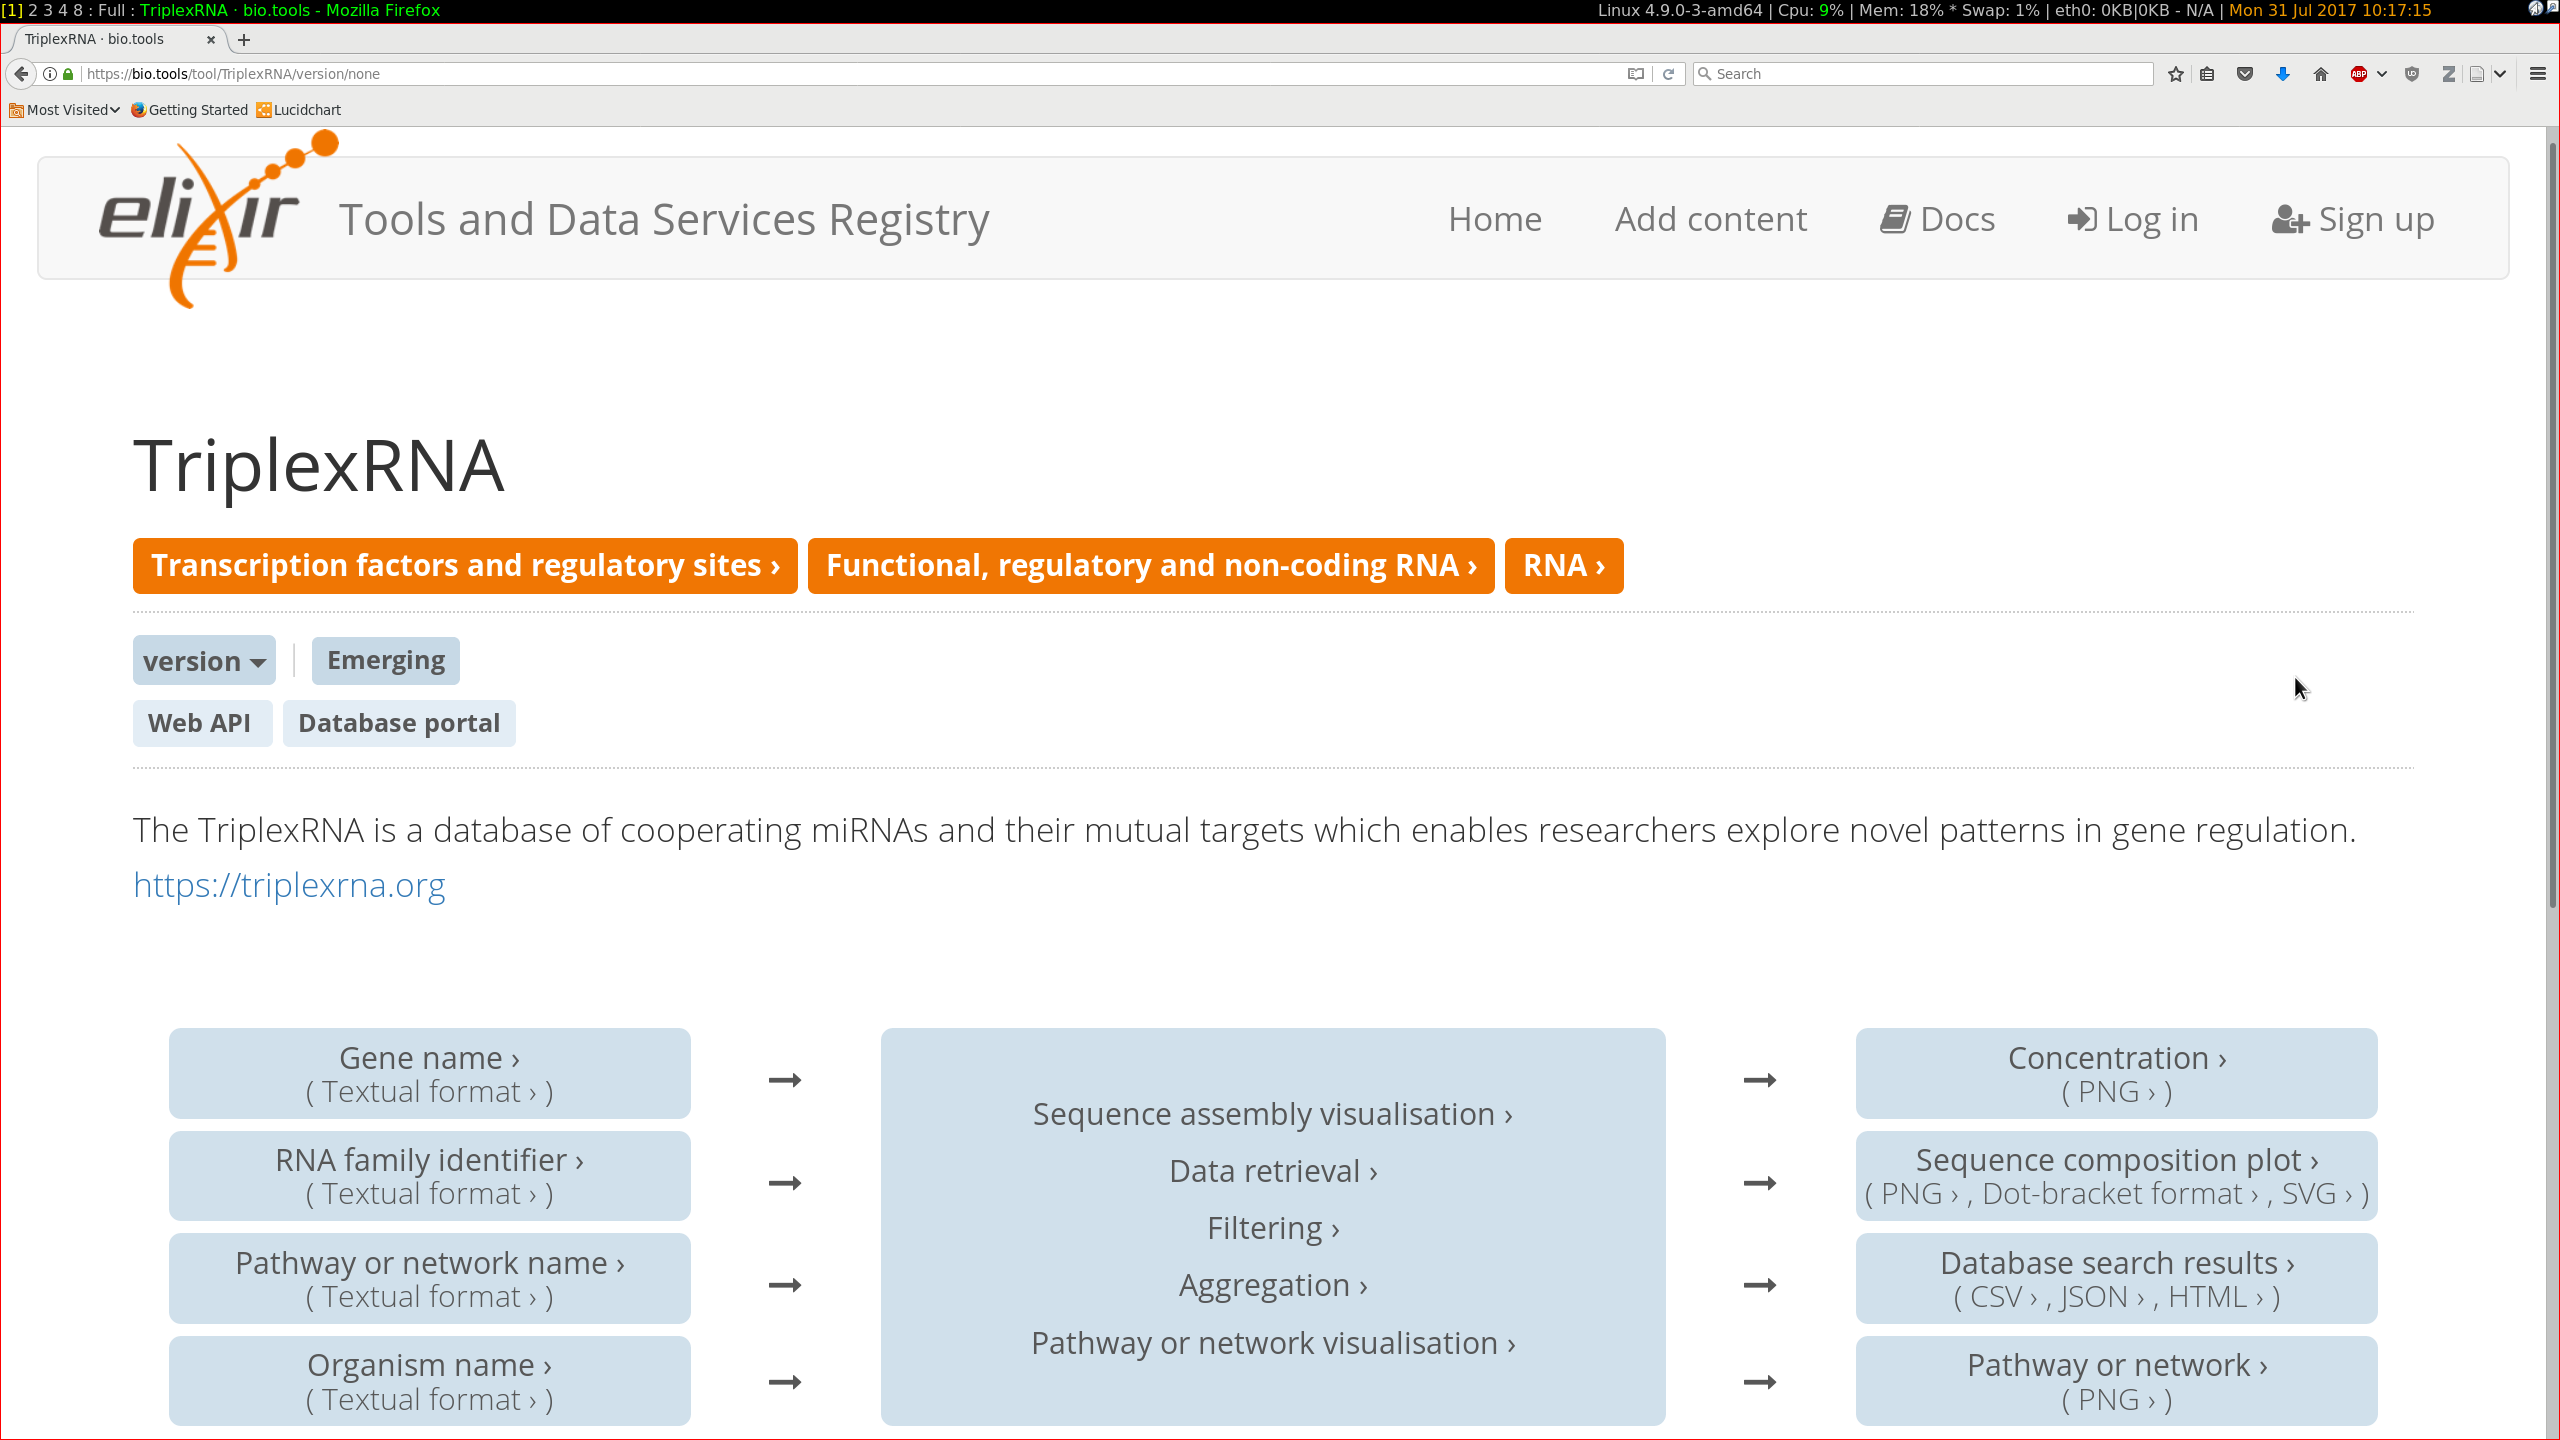
\includegraphics[width=0.90\textwidth]{images/screenshot_biotools_edam}
  \end{center}
\end{frame}

\begin{frame}
  \frametitle{\five}
  \vspace{0.1cm}
  These components will enable us to chain tools on the basis of their functionalities, in/out file formats, and pertinence within a specific kind of data-driven research topic, be it RNA-Seq, Epigenetic analysis, and so on
  \vspace{-0.2cm}
  \begin{center}
    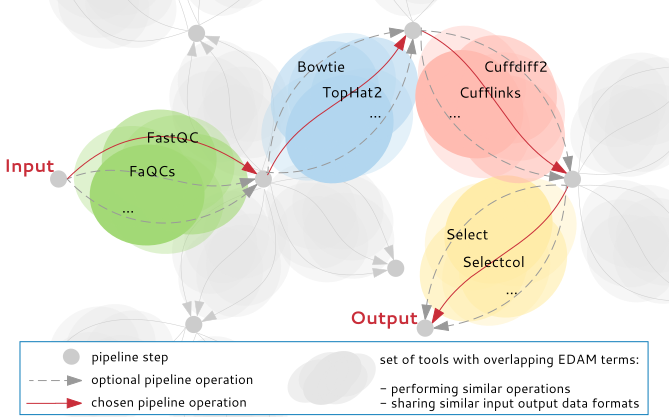
\includegraphics[width=0.80\textwidth]{images/recommendation_system}
  \end{center}
\end{frame}



%
% acknowledgments
%
\begin{frame}
  \frametitle{Acknowledgments}
  \begin{columns}
    \begin{column}{0.5\textwidth}
      \begin{center}
        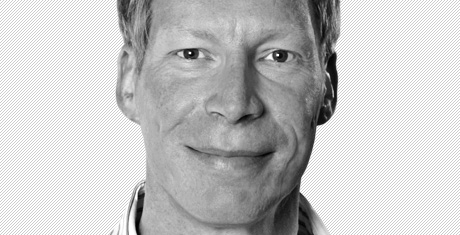
\includegraphics[width=0.70\textwidth]{images/sbi_olaf}
      \end{center}
      \vspace{-0.8cm}
      \begin{center}
        Olaf Wolkenhauer
      \end{center}
      \vspace{-0.1cm}
      \begin{center}
        
\includegraphics[width=0.70\textwidth]{images/sbi_markus}
      \end{center}
      \vspace{-0.8cm}
      \begin{center}
        Markus Wolfien
      \end{center}
    \end{column}
    \begin{column}{0.5\textwidth}
      \vspace{0.5cm}
      \begin{center}
        
\includegraphics[width=0.70\textwidth]{images/logo_bmbf}
      \end{center}
      \vspace{0.2cm}
      \begin{center}
        
\includegraphics[width=0.70\textwidth]{images/logo_denbi}
      \end{center}
      \begin{center}
        
\includegraphics[width=0.70\textwidth]{images/logo_destair}
      \end{center}
    \end{column}
  \end{columns}
\end{frame}

\end{document}
